\chapter{Einführung}
%%===========================================================
Auf der ganzen Welt brachten die vergangenen Jahre eine Fortführung des hohen Wachstum des Online Einzelhandels. Der Umsatz stieg um über 20 Prozente weltweit im Jahr 2014 auf fast 840 Milliarden US-Dollar, da Online-Händler weiter in neuen Regionen ausgebaut haben und die physischen Einzelhändler durch E-Commerce in neuen Märkten eingedrungen sind \citep{HanaBen-Shabat2015}. Das schnelle Wachstum des E-Commerce-Markt hat umfangreiche Forschung angetrieben, um die Meinungen der Konsumenten zu dem Online Handel zu verstehen \citep{tong2010cross}.

Im Online Handel können die Meinungen der Konsumenten einfach als eine Form der \ac{OCRs} erreicht werden. Mit dieser \ac{OCRs} können eine große Menge an Proben ohne Beschränkung von Zeit und Ort erhalten werden. Anders als traditionelle Umfrage und Fragebogen, sind \ac{OCRs} eine spontane Rückmeldung \citep{lu2015understanding}. Während in den meisten Studien eine Probe von Hunderten Menschen verwendet wird, die Meinungen der Konsumenten zu studieren, könnte ein beliebtes Produkt Tausende von \ac{OCRs} haben. Wegen des Wachstums des E-Commerce werden eine enorme Menge der \ac{OCRs} erzeugt.

Es gibt schon viele Forschungen über die \ac{OCRs}. Viele Studien haben die Wichtigkeit der \ac{OCRs} diskutiert, und einige Studien haben schon versucht, die nützliche Information aus die \ac{OCRs} zu extrahieren. In der Mehrheit dieser Studien werden die \ac{OCRs} in zwei Teile unterteilt: der numerische Teil und der schriftliche Teil. Diese Studien fokussieren sich mehr über den numerischen Teil aber der schriftliche Teil von den \ac{OCRs} wird ignoriert, trotzdem der schriftliche Teil mehrere Information erhält.

Sentiment Analyse ist ein Teilgebiet des Text Minings, die die Menschen ermöglicht, die Meinungen von Menschen durch das Text der \ac{OCRs} zu verstehen, ohne manuell das Text durchzulesen und zusammenzufassen. Es ist wichtig, dass die Sentiment Analyse automatisch die Meinungen und die Gefühle vom Text identifizieren könnte. Durch die Sentiment Analyse kann man die Meinungen der Kunden in dem Text der \ac{OCRs} statistisch rechnen, damit man die Gesamtsituationen der Meinungen bewerten kann.

Diese Gesamtsituation ist nützlich, besonders für die kulturübergreifende Forschung. Im Vergleich mit den Gesamtsituationen von verschiedenen Ländern kann man die kulturelle Einflüsse auf die Konsumentenverhalten besser erkennen. Trotz der Tatsache, dass die Unterschiede in der nationalen Kultur das Konsumentenverhalten beeinflussen könnten, haben die meisten Forschungen über die \ac{OCRs} die Wirkung von der Kultur ignoriert \citep{gefen2006need}.

Diese Arbeit macht einen kulturübergreifenden Vergleich zwischen Deutschland und China. Gemeinsam haben die deutschen \acs{B2C}-Mehrkanal-Online- und Versandhandel einen Umsatz von über 49 Milliarden Euro im Jahr 2014. E-Commerce erwirtschaftete mehr als 85 Prozent des gesamten Branchenumsatzes. In Deutschland repräsentierte der Sektor des elektronischen Handels neun Prozent der gesamten Einzelhandelbranche des Landes im Jahr 2014 mit der positiven Tendenz. \citep{Spath2015}

Die chinesischen Online-Käufer sind anspruchsvoll mit gut entwickelten Markenbewusstsein und Vertrauen in der größten Namen, einschließlich inländischer Führer wie Tmall und JD.com sowie internationaler wie Amazon und eBay. In China erstellen die chinesischen Käufer in dem elektronischen Handel ein kulturelles Phänomen,vor allem am Ledigen Tag (11. November), die ähnlich wie Cyber Monday in den USA ist. Alibaba (Plattformbetreiber von Tmall) hat 9,3 Milliarden Dollar Umsatz am Ledigen Tag 2014 gemeldet, entsprechend ungefähr sieben Prozent des Gesamtjahresumsatz des Landes. \citep{HanaBen-Shabat2015}

Online Textileinzelhandel ist eine der größten Kategorien im elektronischen Handel mit starker Wachstumsrate. Online Textileinzelhandel ist eine der größten Branchen in elektronischen Handel aber es gibt nicht so viele kulturübergreifenden Forschungen darüber, insbesondere im Bereich \acl{OCRs}. \ac{OCRs} werden die Kaufentscheidungen stark beeinflussen. Zum Beispiel, wollen 40 Prozent der Online Käufer in China unmittelbar ``kaufen oder nicht kaufen'' Beratungen und Bewertungen \citep{HanaBen-Shabat2015}. Deutschland und China, haben große Unterschiede in den Kulturen, und die beiden Länder sind wichtig für die Wirtschaft der Welt, aber es gibt anhand noch keine Forschungen, die über die Unterschiede von Kulturen und \ac{OCRs} zwischen den beiden Ländern diskutiert.
%%===========================================================
\section{Forschungsfragen}
%%===========================================================
Diese Arbeit wird die folgende Forschungsfragen diskutiert:
\begin{enumerate}
	\item Wie sollten die \acl{OCRs} von China und Deutschland sein, basierend auf den theoretischen Grundlagen? 
	\item Welche Unterschiede haben die \acl{OCRs} von China und Deutschland in der Tat durch Sentiment Analyse? 
	\item Welche Unterschiede gibt es zwischen der Tat und Theorie? Warum?
	\item Welche Wirkungen gibt es von dieser Unterschiede der \acl{OCRs} in den beiden Ländern?
\end{enumerate}
%%===========================================================
\section{Die Struktur der Arbeit}
%%===========================================================
Um diese Forschungsfragen zu antworten, wird die Arbeit in der Struktur geschrieben, die in der Abbildung \ref{fig:struktur} gezeigt wird. Erst werden die deutschen und chinesischen \ac{OCRs} gesammelt, dann werden sie durch die Sentiment Analyse analysiert und die Ergebnisse werden durch statistischen Maßnahmen verglichen. Die Unterschiede werden mit den kulturellen Unterschieden diskutiert und begründet. Die Wirkungen von dieser Unterschieden werden auch in verschiedenen Sichten diskutiert.

\begin{figure}[htb]
	\centering
	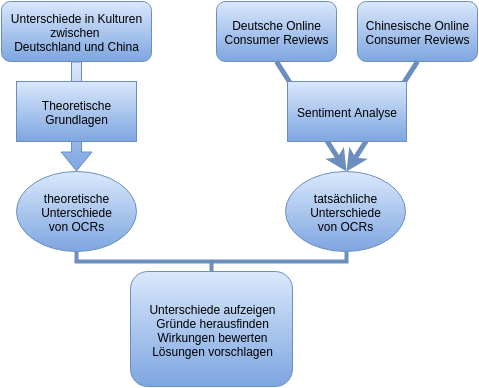
\includegraphics[width=0.85\textwidth]{einfuehrung/struktur}
	\caption[Die Struktur der Arbeit]{Die Struktur der Arbeit (Quelle: Eigene Darstellung)}
	\label{fig:struktur}
\end{figure}

\begin{description}
	\item[Kapitel 2] In Kapitel 2 werden die theoretischen Grundlagen geschrieben. Hier werden erst die \acl{OCRs} vorgestellt, einschließlich des Begriffs und Forschungsstand in der Marketingforschung, der Motive für das Schreiben der \acl{OCRs}, der Wirkungen und \acl{OCRs} im Textileinzelhandel. Danach werden die Definition, der Ablauf, der Kernprozess und der in dieser Arbeit verwendete Algorithmus von der Sentiment Analyse eingeführt. Durch die Sentiment Analyse haben die \acl{OCRs} einige statistischen Attribute. Dann wird das sechsdimensionale Modell für Deutschland und China von \citeauthor{hofstede2013interkulturelle} vorgestellt, und die Unterschiede zwischen den beiden Ländern werden herausgefunden. Die relevante Forschungsergibnisse werden aufgeführt, die meisten in dem kulturübergreifenden Bereich sind. Basierend auf diesen theoretischen Grundlagen werden vier Hypothese für die Forschungsfragen aufgestellt. 
	\item[Kapitel 3] Kapitel 3 stellt den Prozess der Datensammlung und Textverarbeitung vor. Zwei \ac{B2C} Plattformen Amazon Deutschland und Tmall (China) werden als die Datenquellen sein. Vier unterschiedlichen Sportkleidungen aus Adidas, Nike und Puma werden als die Untersuchungsobjekte ausgewählt. Diese Untersuchungsobjekte müssen bestimmte Bedingungen erfüllen. Weiterhin werden die technischen Werkzeuge in der Datensammlung vorgestellt und der Datensammlungsprozess aus beiden Plattformen dokumentiert. Nach der Datensammlung werden die Rohdaten vor der Analyse bestimmte Verarbeitungen gemacht und die chinesischen Rohdaten werden durch eine Übersetzungsmaschine auf Deutsch übersetzt, damit die Ergebnisse besser verglichen werden könnten. Die Einflüsse von der Übersetzung werden auch in diesem Abschnitt diskutiert.
	\item[Kapitel 4] In diesem Kapitel werden die empirischen Ergebnisse deskriptiv erst gezeigt. Vor der Prüfungen der Hypothesen, muss man erst bestimmen, ob die \acl{OCRs} statistisch normal verteilt sind. Dies ist die Basis, welche Prüfverfahren für die Hypothesen sollte man auswählen. Je nach der Überprüfung der vier Hypothesen wird das Ergebnis gezeigt.
	\item[Kapitel 5] In Kapitel 5 wird erst die Zusammenhängen von den kulturellen Dimensionen und den Ergebnissen diskutiert, um die Gründe der Unterschiede von China und Deutschland zu entdecken. Und die Motive für das Schreiben der \acl{OCRs} und die Wirkungen der Ergebnisse in Konsumenten-, Unternehmen- und Plattformenbetreiberssicht werden auch diskutiert.  
	\item[Kapitel 6] In diesem Kapitel wird die Arbeit zusammengefasst, und einige Limitationen auf unterschiedlichen Gründen werden aufgestellt. Darüber hinaus wird die Ausblick auf die zukünftigen Forschung geführt.
\end{description} 

